\documentclass[a4paper,ngerman]{scrartcl}

\usepackage{amsmath}
\usepackage{amsfonts}
\usepackage{amssymb}
\usepackage[utf8]{inputenc}
\usepackage{graphicx}
\usepackage[ngerman]{babel}
\usepackage{hyperref}
\usepackage{float}
\usepackage{caption}
\usepackage{subcaption}
\usepackage{multirow}  %for tables
\usepackage{icomma} % Handle german comma as decimal point in numbers
\usepackage{units,siunitx} % Write units with correct spacing
\usepackage{upgreek} % provide non-italic greek letters
\usepackage{url}
\usepackage{hepnames} % hier gibt es symbole fuer unterschiedliche elementarteilchen, aber dieses paket gibts nicht im poolraum

%\usepackage{subfig}

% Formatting of table & figure captions
\captionsetup{font={sf,footnotesize},labelfont=bf,textfont=sl,skip=6pt}

\sisetup{locale = DE, % use "," as decimal point instead of "."
  exponent-product={\cdot},% used \cdot in front of 10^x
  separate-uncertainty} % give out uncertainty with \pm instead of in brackets

\setlength{\abovecaptionskip}{6pt}
\setlength{\belowcaptionskip}{0pt}

\title{Elementarteilchen 2\\Vorbereitung}
\date{\today}
\author{Michel Rausch, Michael Eliachevitch}

\begin{document}

\maketitle
\tableofcontents
\newpage

\section{Einleitung}

\section{Das DELPHI Experiment am LEP}
\label{sec:delphi}

\begin{figure}
\centering
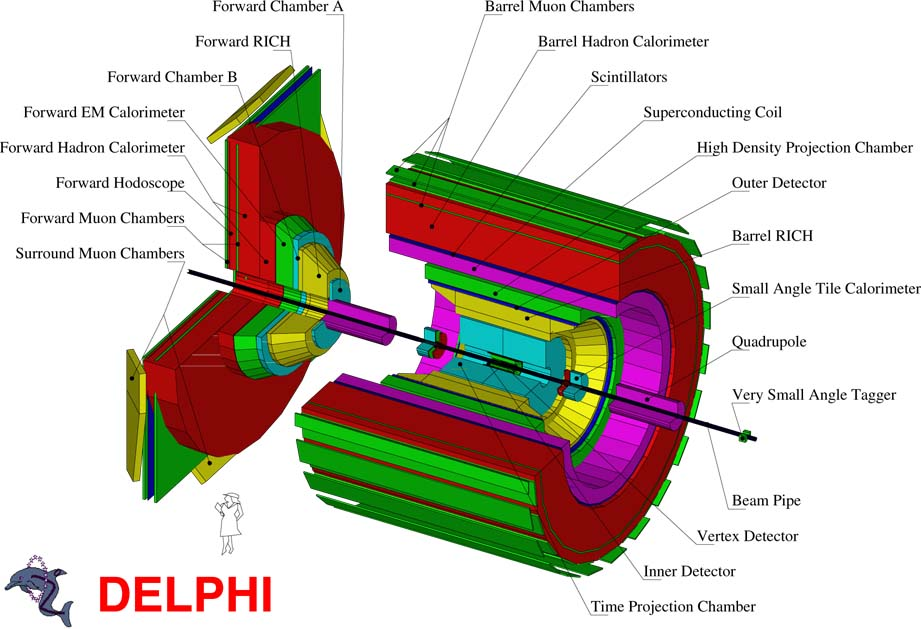
\includegraphics[width=\textwidth]{abbildungen/delphi_big.png}
\caption{\textbf{Aufbau des DELPHI-Detektors mit einer sichtbaren Endkappe [\ref{ref:hands-on}].} 
Die Bestandteile des Detektors sind farblich gekennzeichnet und benannt.
Links ist eine der beiden Endkappen zu sehen, die andere wurde zur Übersichtlichkeit ausgeblendet.
Rechts im Bild ist der zylindrische zentrale Teil mit Strahlengang gezeigt. 
}
\label{fig:delphi_big}
\end{figure}





\begin{figure}
\centering
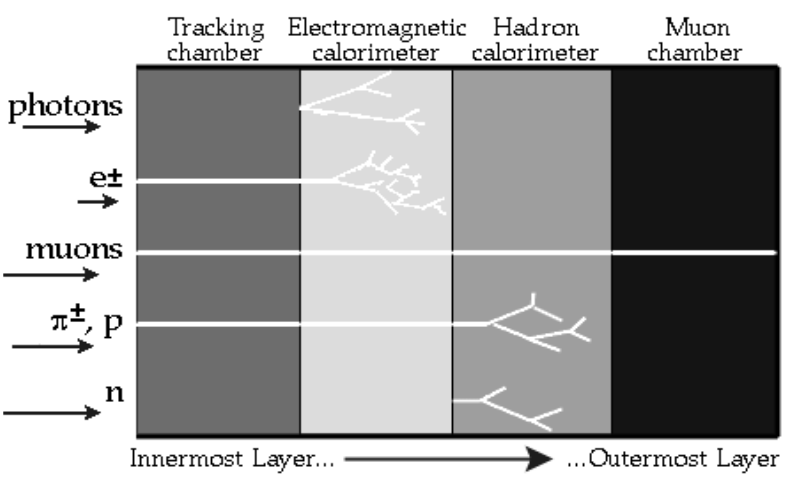
\includegraphics[width=0.7\textwidth]{abbildungen/delphi_schichten.png}
\caption{\textbf{Übersicht der Signaturen nachweisbarer Teilchen in den Subdetektoren [\ref{ref:BB}].} 
}
\label{fig:delphi_schichten}
\end{figure}


\section{Mögliche Zerfälle und Bestimmung der Zerfallsbreiten und Kopplungskonstanten}
\label{sec:zerfaelle}


\section{Das Scannen von Ereignissen mit "`Fireworks"' und Beispielzerfälle}
\label{sec:scannen}

\section{Quellen}
\begin{enumerate}
\item Blaues Buch \label{ref:BB}
% Quelle fuer PDG-Angaben: (noch nicht genutzt, daher auskommentiert)
% \item K.A. Olive et al. (Particle Data Group), Chin. Phys. C, 38, 090001 (2014). \label{ref:pdg14}
\item \url{http://hands-on-cern.physto.se/hoc_v21en/index.html} (25.1.2015)\label{ref:hands-on}
\end{enumerate}



\end{document}
